\documentclass[lang=en,11pt]{../simplebook}

\usepackage{hologo}
\usepackage{listings}

\renewcommand{\ttdefault}{cmtt}
\lstdefinestyle{mystyle}{
basicstyle=%
    \ttfamily
    \lst@ifdisplaystyle\small\fi
}

\lstset{basicstyle=\ttfamily,style=mystyle,breaklines=true}

\definecolor{lightgrey}{rgb}{0.9,0.9,0.9}
\definecolor{frenchplum}{RGB}{190,20,83}
\lstset{language=[LaTeX]TeX,
texcsstyle=*\color{winered},
numbers=none,
mathescape=false,
breaklines=true,
keywordstyle=\color{winered},
commentstyle=\color{gray},
emph={simplepaper,fontenc,fontspec,cnfont,xeCJK,citestyle,FiraMono,xunicode,figure,fig,image,img,table,itemize,enumerate,ctex,microtype,description,times,booktabs,tabular,PDFLaTeX,XeLaTeX,type1cm,BibTeX,color,mode,lang,amsthm,tcolorbox,titlestyle,cite,ctex,listings,base,math,scheme,toc,esint,chinesefont,amsmath,bibstyle,natbib,pgfornament,addbibresource,printbibliography},
emphstyle={\color{frenchplum}},
morekeywords={DeclareSymbolFont,SetSymbolFont,toprule,midrule,bottomrule,institute,version,includegraphics,setmainfont,setsansfont,setmonofont ,setCJKmainfont,setCJKsansfont,setCJKmonofont,RequirePackage,figref,tabref,email,maketitle,keywords,definecolor,bottominfo,logo,cover,subtitle,appendix,chapter,section,hypersetup,mainmatter,frontmatter,tableofcontents,heiti,kaishu,lstset,pagecolor,zhnumber,part,equote,bioinfo,datechange,listofchange,lvert,lastpage,songti,heiti,fangsong,setCJKfamilyfont,textbf,thmcnt,colorlet,usesamecnt},
frame=single,
tabsize=2,
rulecolor=\color{ecolor},
framerule=0.2pt,
columns=flexible,
% backgroundcolor=\color{lightgrey}
}
\renewcommand\ttdefault{lmtt}

\title{SimpleBook Book Template v1.0}
\subtitle{\LaTeX{} template based on ElegantBook}

\author{Fenglielie}
% \institute{None}
\date{2024-03-22}
\bottominfo{}
\cover{legao.jpg}
%\logo{logo-blue.png}

\setcounter{tocdepth}{2}

\RequirePackage[backend=biber,citestyle=numeric-comp,bibstyle=numeric]{biblatex}
\addbibresource[location=local]{reference.bib}

\begin{document}

\maketitle

\frontmatter

\chapter*{Preface}

SimpleBook is a note template modified based on \href{https://github.com/ElegantLaTeX/ElegantBook}{ElegantBook}. ElegantBook is a well-known open-source book template,
but the author ceased updating it on January 1, 2023.
SimpleBook is based on its final version, which has been organized and simplified: most of the fancy beautification configurations have been removed,
and the code retained in ElegantBook for version compatibility has been cleaned up.

The project is hosted on GitHub: \href{https://github.com/fenglielie/simplebook/}{https://github.com/fenglielie/simplebook/}.


\tableofcontents

\mainmatter

\chapter{Configuration}

SimpleBook supports two compilation methods: \hologo{pdfLaTeX} and \hologo{XeLaTeX}.
It supports two modes: Chinese and English. In English mode, any compilation method can be used, while in Chinese mode, \hologo{XeLaTeX} must be used.
When using the SimpleBook document class, the main options are as follows:

\begin{enumerate}
    \item Language: Chinese (cn, default) or English (en).
    \item Color: Determines the theme color, including blue (default) and black.
    \item Chinese fonts: Determines the Chinese fonts, including several default options provided by ctex and open-source fonts such as Fangzheng and Source Han Sans. See below for details.
\end{enumerate}


\begin{remark}
    The options for the document class can be specified either in full key-value pairs, for example \lstinline{device=normal},
    or directly by using the option name, such as \lstinline{normal}. Multiple options can be set consecutively, and in any order.
\end{remark}

\section{Language}
This template includes two basic language environments: \lstinline{lang=cn} (Chinese) and \lstinline{lang=en} (English),
with Chinese being the default. Changing the language environment will affect the captions of figures and tables, structural words (such as table of contents, bibliography, etc.),
and the lead words in theorem environments (such as theorem, lemma, etc.). The language mode can be enabled as follows:
\begin{lstlisting}
\documentclass[en]{simplebook}
\documentclass[lang=en]{simplebook}
\end{lstlisting}


\section{Color}

The default theme color of this template is the blue-green tone \lstinline{blue}, which can be changed to \lstinline{black} for an all-black theme.
If custom colors are needed, choose the \lstinline{nocolor} option or use \lstinline{color=nocolor},
and then define the colors \lstinline{ecolor}, \lstinline{main}, \lstinline{second}, and \lstinline{third} in the preamble as follows:
\begin{lstlisting}[tabsize=4]
\definecolor{ecolor}{RGB}{0,0,0}
\definecolor{main}{RGB}{70,70,70}
\definecolor{second}{RGB}{115,45,2}
\definecolor{third}{RGB}{0,80,80}
\end{lstlisting}

\section{Chinese Fonts}

Please refer to the Chinese documentation for the explanation of this section.


\section{Cover Information}

Currently, the cover supports many elements, and all cover elements, including \lstinline{\title}, can be left empty.

\begin{itemize}
    \item \textbf{Title}: \lstinline|\title|
    \item \textbf{Subtitle}: \lstinline|\subtitle|
    \item \textbf{Author}: \lstinline|\author|
    \item \textbf{Institute}: \lstinline|\institute|
    \item \textbf{Date}: \lstinline|\date|
    \item \textbf{Bottom Info}: \lstinline|\bottominfo|
    \item \textbf{Cover}: \lstinline|\cover|
    \item \textbf{Logo}: \lstinline|\logo|
\end{itemize}

The cover image must be \textbf{strictly} replaced with an image of size $1280 \times 1024$:
\begin{lstlisting}
\cover{demo.jpg}
\end{lstlisting}
The color of the block in the middle of the cover can be modified using the following command:
\begin{lstlisting}
\definecolor{customcolor}{RGB}{32,178,170}
\colorlet{coverlinecolor}{customcolor}
\end{lstlisting}
A logo can be added to the bottom right corner of the cover. The logo image should have a ratio of 1:1, and it can be omitted:
\begin{lstlisting}
\logo{demo.jpg}
\end{lstlisting}


\section{References}

The original ElegantBook template includes the section for references: using the Biblatex package and supporting style passing through parameters. However, for personal reasons, this part has been completely removed, and configuration needs to be done manually when referencing is required.

The basic usage of traditional BibTeX is as follows:
\begin{enumerate}
    \item Specify the style in the preamble, for example, \lstinline|\bibliographystyle{plain}|.
    \item Use \lstinline|\bibliography{reference}| at the location where the bibliography list is to be displayed. Here, it is assumed that the bibliography file is named reference.bib.
\end{enumerate}
An example is as follows:
\begin{lstlisting}[frame=single]
\documentclass{article}
\bibliographystyle{plain}

\begin{document}

According to Einstein's theory of relativity \cite{einstein1905}...

\bibliography{reference} % reference.bib

\end{document}
\end{lstlisting}

The basic usage of modern Biblatex is as follows:
\begin{enumerate}
    \item Import the biblatex package in the preamble, where you can specify the style and backend.
    \item Load the bibliography file in the preamble, for example, \lstinline|\addbibresource[location=local]{reference.bib}|. Here, it is assumed that the bibliography file is named reference.bib.
    \item Use \lstinline|\printbibliography| at the location where the bibliography list is to be displayed.
\end{enumerate}
An example is as follows:
\begin{lstlisting}[frame=single]
\documentclass{article}
\usepackage[style=authoryear]{biblatex}
\addbibresource{reference.bib} % reference.bib

\begin{document}

According to Einstein's theory of relativity \parencite{einstein1905}...

\printbibliography[title={References}]

\end{document}
\end{lstlisting}


\section{Mathematical Environments}

This template supports common mathematical theorem environments:

\begin{itemize}
    \item \textit{Theorem-like environments}, which include both title and content. All theorem-like environments are numbered according to chapter numbers. There are two types based on formatting:
          \begin{itemize}
              \item \textcolor{main}{\textbf{definition}} environment, with color \textcolor{main}{main};
              \item \textcolor{second}{\textbf{theorem, lemma, corollary, proposition}} environments, with color \textcolor{second}{second}.
          \end{itemize}
    \item \textit{Examples}, including \textbf{\color{main}{example}}, \textbf{\color{main}{problem}}, and \textbf{\color{main}{exercise}} environments (corresponding to example, problem, and exercise). They are automatically numbered, with numbering based on chapters.
    \item \textit{Notes and Remarks}, including \textbf{\color{third}{note}}, \textbf{\color{third}{remark}}, and \textbf{\color{third}{solution}} environments, without numbering.
\end{itemize}

Each theorem-like environment has a starred version: \textcolor{main}{\textbf{definition*}}, \textcolor{second}{\textbf{theorem*}}, \textcolor{second}{\textbf{lemma*}}, \textcolor{second}{\textbf{corollary*}}, \textcolor{second}{\textbf{proposition*}}. Starred theorem-like environments are unnumbered. Additionally, there is a \textbf{\color{third}{proof}} environment.

Usage of theorem-like environments is as follows:

\begin{lstlisting}
\begin{theorem}[theorem name]\label{thm:label}
  This is a named theorem with a label. You can reference this theorem using \ref{thm:label}.
\end{theorem}

\begin{theorem}[theorem name]
  This is a named theorem.
\end{theorem}
\end{lstlisting}

The other three environments do not have options and can be used directly. For example, the usage and effect of the \lstinline{example} environment are as follows:

\begin{lstlisting}
\begin{example}
   This is the content of the example environment.
\end{example}
\end{lstlisting}


\begin{remark}
    The original ElegantBook supported two modes for mathematical theorem environments: fancy and simple. However, I personally felt that the colorful boxes in fancy mode were too fancy, so I chose to remove them directly.
\end{remark}



\chapter{Writing Sample}

\begin{theorem}[Fubini's Theorem]\label{thm:fubi}
    If $f(x,y)$ is a non-negative measurable function on $\mathcal{R}^p\times\mathcal{R}^q$,
    then for almost every $x\in \mathcal{R}^p$, $f(x,y)$ as a function of $y$ is non-negative and measurable on $\mathcal{R}^q$,
    and $g(x)=\int_{\mathcal{R}^q}f(x,y) dy$ is non-negative and measurable on $\mathcal{R}^p$. Moreover,
    \begin{equation}\label{eq:461}
        \int_{\mathcal{R}^p\times\mathcal{R}^q} f(x,y) dxdy=\int_{\mathcal{R}^p}\left(\int_{\mathcal{R}^q}f(x,y)dy\right)dx.
    \end{equation}
\end{theorem}


\begin{theorem}
    For the Burgers' equation, assuming a smooth initial value $u_0(x)$, and if there exist some points where $u_0'(x) < 0$,
    then the exact solution first intersects at the characteristic lines at time $T_b$, and infinite slope (discontinuity, shock) appears at time $T_b$.
    \[
        T_b = \frac{-1}{\min u_0'(x)}
    \]
\end{theorem}
\begin{proof}
    The proof is divided into two parts: first, prove that the characteristic lines first intersect at time $T_b$, and then prove that infinite slope appears at time $T_b$, details of the proof are omitted.
\end{proof}


\begin{lemma}[Harten's Lemma]
    If the difference scheme can be formulated as follows
    \[
        v_j^{n+1} = v_j^n - C_{j-1/2}(v_j^n - v_{j-1}^n) + D_{j+1/2}(v_{j+1}^n - v_j^n)
    \]
    and it holds everywhere
    \[
        C_{j+1/2} \ge 0, D_{j+1/2} \ge 0, C_{j+1/2} + D_{j+1/2} \le 1, \forall j
    \]
    then it is a TVD scheme.
\end{lemma}

\begin{proposition}
    The following two conclusions are equivalent:
    \begin{enumerate}
        \item There exists a constant $\delta >0$ such that all eigenvalues of $A$ satisfy $\Re\, \lambda \ge \delta$; (parabolic definition)
        \item There exists a constant $\delta >0$ such that $A + A^* \ge \delta I$.
    \end{enumerate}
\end{proposition}

\begin{corollary}
    Monotone schemes must be TVD schemes, TVD schemes must be monotonicity-preserving schemes, but the converse is not true.
    In the context of linear difference schemes, monotone schemes, TVD schemes, and monotonicity-preserving schemes are equivalent concepts.
\end{corollary}

\begin{definition}[Conservative Scheme]
    A difference scheme is called a conservative scheme if it can be formulated as follows
    \begin{equation}
        v_{j}^{n+1} = v_j^n - \frac{\Delta t}{\Delta x}\left(
        \hat{f}_{j+1/2}^n - \hat{f}_{j-1/2}^n
        \right) \tag{$*$}
    \end{equation}
    where $\hat{f}_{j+\frac12}$ is called the numerical flux, with the expression $\hat{f}_{j+\frac12} = \hat{f}(v_{j-r},\cdots,v_{j+s})$,
    and satisfies
    \begin{enumerate}
        \item Continuity: $\hat{f}$ is locally Lipschitz continuous with respect to each variable
        \item Compatibility: $\hat{f}(v,\dots,v) = f(v)$
    \end{enumerate}
\end{definition}

\begin{example}
    The characteristic lines of the Burgers' equation $u_t + u u_x = 0$ satisfy
    \begin{equation}
        \frac{d x}{d t} = f'(u_0(x_0)) = u_0(x_0)
    \end{equation}
    The characteristic lines are straight lines in the $x\!-\!t$ plane
    \begin{equation}
        x = x_0 + u_0(x_0) t \label{eq:1}
    \end{equation}
\end{example}

Below are examples of images and tables.
\figref{fig:1} presents a typical exact solution of the Burgers' equation, obtained by solving the nonlinear equation \eqref{eq:1};
\tabref{tab:1} presents a comparison of a set of numerical algorithms, including errors and orders.

\begin{figure}[htbp]
    \centering
    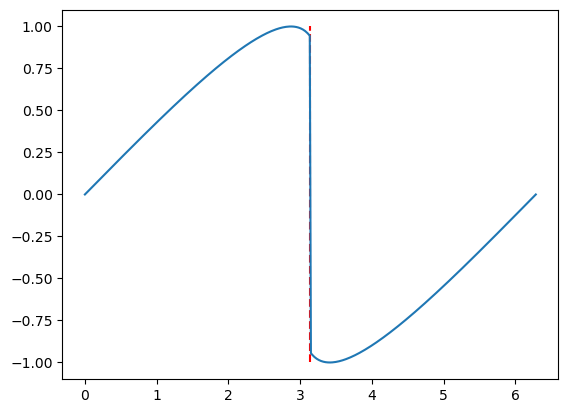
\includegraphics[width=.6\textwidth]{burgers.png}
    \caption{Solution of Burgers' equation}
    \label{fig:1}
\end{figure}

\begin{table}[ht]
    \centering
    \caption{Computational Results}\label{tab:1}
    \begin{tabular}{c|c|ccccc}
        \hline
                              &                & N=25     & N=50       & N=100      & N=200      & N=400      \\
        \hline
        \multirow{4}{*}{FTCS} & Error          & 2.8e-03  & 7.1121e-04 & 1.7821e-04 & 4.4559e-05 & 1.1139e-05 \\
                              & Order of Error & -        & 1.97       & 1.99       & 2.00       & 2.00       \\
                              & Time/s         & 0.009449 & 0.009827   & 0.087355   & 0.840438   & 33.303874  \\
        \hline
        \multirow{4}{*}{SVD}  & Error          & 2.8e-03  & 7.1121e-04 & 1.7847e-04 & 4.4615e-05 & 1.1153e-05 \\
                              & Order of Error & -        & 1.97       & 1.99       & 2.00       & 2.00       \\
                              & Time/s         & 0.016365 & 0.010492   & 0.034441   & 0.205993   & 1.431576   \\
        \hline
    \end{tabular}
\end{table}


\begin{problem}
Determine the order of accuracy of the following difference
equations to the partial differential equation
\begin{equation*}
    u_t+au_x=0
\end{equation*}
\begin{equation*}
    v^{n+1}_k=v^{n-1}_k-R\delta_0u^n_k+\frac{R}{6}\delta^2\delta_0u^n_k
\end{equation*}
\end{problem}
\begin{solution}
    The truncation error is
    \begin{equation*}
        \begin{aligned}
            T^n_k= & \frac{u^{n+1}_k-u^{n-1}_k}{2\Delta t}+\frac{a}{2\Delta x}(u^n_{k+1}-u^n_{k-1})-\frac{a}{12\Delta x}(u^n_{k+2}-2u^n_{k+1}+2u^n_{k-1}-u^n_{k-2}) \\
            =      & (u_t+\frac{\Delta t^2}{6}u_{ttt}+O(\Delta t^4))|^n_k+a(u_x+\frac{\Delta x^2}{6}u_{xxx}+\frac{\Delta x^4}{120}u_{xxxxx}+O(\Delta x^6))|^n_k     \\
                   & -\frac{a}{12}(2\Delta x^2u_{xxx}+\frac{\Delta x^4}{2}u_{xxxxx}+O(\Delta x^6))|^n_k                                                             \\
            =      & O(\Delta t^2+\Delta x^4)
        \end{aligned}
    \end{equation*}
    2nd order in time, 4th order in space.
\end{solution}

\begin{remark}
    This is a remark content test.\footfullcite{lubichProjectorsplittingIntegratorDynamical2014}
\end{remark}

\begin{note}
    This is a note content test.\autocite{kochDynamicalLowRank2007}
\end{note}

Nested unordered lists look like this:
\begin{itemize}
    \item xxx
    \item xxx
          \begin{itemize}
              \item yyy
              \item yyy
                    \begin{itemize}
                        \item zzz
                        \item zzz
                              \begin{itemize}
                                  \item www
                                  \item www
                              \end{itemize}
                    \end{itemize}
          \end{itemize}
\end{itemize}

Nested ordered lists look like this:
\begin{enumerate}
    \item xxx
    \item xxx
          \begin{enumerate}
              \item yyy
              \item yyy
                    \begin{enumerate}
                        \item zzz
                        \item zzz
                              \begin{enumerate}
                                  \item www
                                  \item www
                              \end{enumerate}
                    \end{enumerate}
          \end{enumerate}
\end{enumerate}








\nocite{*}

\printbibliography[heading=bibintoc, title={References}]
\appendix


\chapter{Mathematical Tools}

This appendix covers some of the basic mathematics used in econometrics. We briefly discuss the properties of summation operators, study the properties of linear and some nonlinear equations, and review the ratios and percentages. We also introduce some special functions that are common in econometrics applications, including quadratic functions and natural logarithms. The first four sections require only basic algebraic techniques. The fifth section briefly reviews differential Calculus Although Calculus is not necessary to understand much of this book, it is used in some of the end-of-chapter appendices and in some of the more advanced topics in part 3.

\section{Summation Operator and Description Statistics}

\textbf{Summation Operator} is an abbreviation used to express the summation of numbers, it plays an important role in statistics and econometrics analysis. If $\{x_i: i=1, 2, \ldots, n\}$ is a sequence of $n$ numbers, the summation of the $n$ numbers is:

\begin{equation}
    \sum_{i=1}^n x_i \equiv x_1 + x_2 +\cdots + x_n
\end{equation}


\end{document}
